% !TEX root = ../../prj4projektdokumentation.tex

\section{Software}

I dette afsnit vil softwaren for Måleenheden blive beskrevet. Herunder beskrivelser af det overordnede flow i koden, samt en uddybning af udviklede funktioner til sampling, Fourier-udregninger og Total Harmonic Distortion. 

\subsection{Overordnet beskrivelse}

Softwaren til Måleenheden er allokeret på PSOC. Det overordnede flow i koden er beskrevet i Figur \ref{fig:MEflowchart}. 

Som det første åbnes der for globale interrupts, så der kan modtages receive-interrupts fra UART forbindelsen til Styringsenheden. Herefter inittieres de anvendte blokke i PSOC, herunder ADC og UART. 

Efter initialiseringen går koden i et uendeligt loop hvor der ikke er nogen aktivitet.  Her ventes der på et receive-interrupt fra UART forbindelsen. Ifølge protokollen for kommunikation mellem Måleenhed og Styringsenhed, se kapitel \ref{ch:KomProtokol}, forventes det at rækkefølgen af karakterer der modtages er "A-B-C-D". Denne rækkefølge er afgørende, da sampling og udregning, først starter ved modtagelse af karakteren 'A'. 

Når udregningerne er udført, sendes den udregnede RMS-værdi for den målte strøm, over UART-forbindelsen. Værdien, som er en 16bit integer, sendes i to bytes, henholdsvis MSB og LSB. 

Når de to bytes er sendt til Styringsenheden forlades interruptrutinen, og koden returnerer til det uendelig loop, hvor der ventes på at modtage den næste karakter i rækkefølgen. 

Ved modtagelse af de efterfølgende karakterer sendes værdierne for henholdsvis spænding, THD og Power Factor. 


\begin{figure}[H] % (alternativt [H])
	\centering
	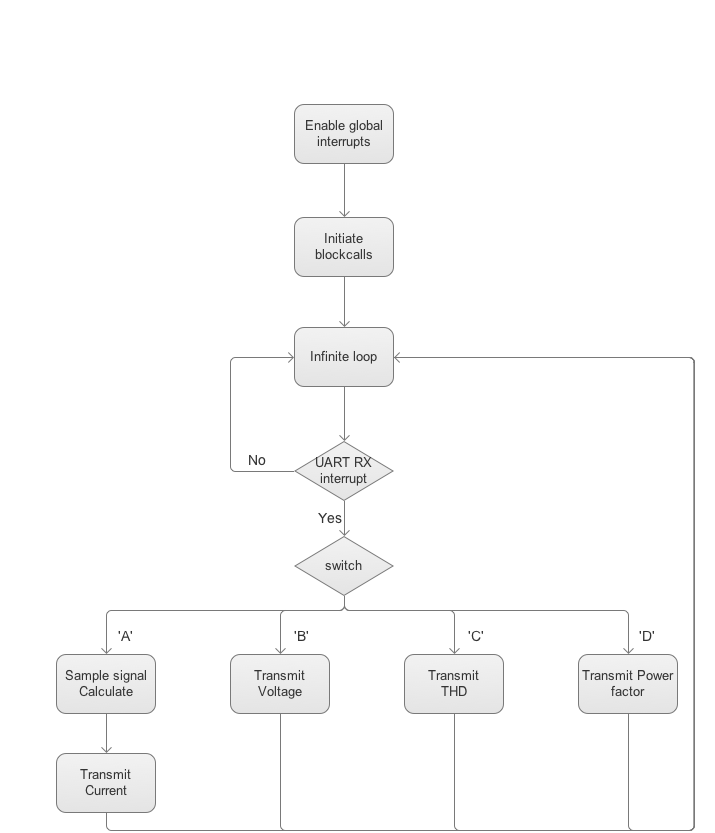
\includegraphics[width=0.7\textwidth]{Figure/MEflowchart.png}
	\caption{Overordnet flowchart for software på Måleenhed}
	\label{fig:MEflowchart}
\end{figure}

